\chapter{Importing and exporting}
\label{txt:importExport}
Importing and exporting of dendro data in Tellervo is provided through the TRiCYCLE libraries.  TRiCYCLE is a universal dendro data conversion application for converting back and forth between 22 supported data formats \citep{tricycle}.  The open source libraries that provide the functionality to TRiCYCLE are incorporated directly into Tellervo providing support for all these formats.  

\begin{table*}[htbp]
\centering
\label{txt:formatList}
\index{File formats}
\begin{tabular*}{0.8\textwidth}{ll}
\toprule
Belfast Apple & ODF Spreadsheet \\
Belfast Archive & Oxford \\
Besancon (including SYLPHE variants) &   PAST4\\
CATRAS & Sheffield D-Format (Dendro for Windows)\\
Comma delimited text files (CSV) &  Topham \\
Tellervo Legacy &  TRiDaS\\
DendroDB & TRIMS\\
Heidelberg (TSAP-Win) &  Tucson (RWL and CRN)\\
Microsoft Excel 97/2000/XP& Tucson Compact\\
Microsoft Excel 2007 & VFormat\\
Nottingham &  WinDENDRO\\
\bottomrule
\end{tabular*}
\caption{List of the twenty-two formats supported by Tellervo. See appendices \ref{txt:fileFormatsStart}--\ref{txt:fileFormatsLast} (pages \pageref{txt:fileFormatsStart}--\pageref{txt:fileFormatsEnd}) for full descriptions.}
\end{table*}



\section{Exporting data}
\index{Export!Data}
Exporting data is initiated by the \menutwo{File}{Export data menu}.  If this is called from the main Tellervo data window, it will export the current series.  If it is called from the Tellervo home screen, then it will present you with the database browser and allow you to pick one or more series to export.  If you use the menu from within the main data editor then it will export 

\begin{SCfigure}
  \centering
    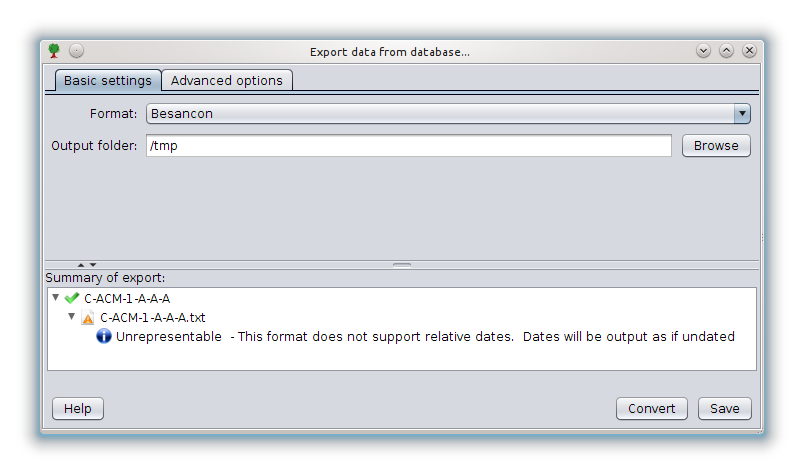
\includegraphics[width=0.7\textwidth]{Images/exportdata1.png}
    \caption{Screen showing a series that has been exported to Besan\c{c}on format.  In the summary of the export at the bottom of the screen you can see the warning to the user that this format does not have the ability to represent relative dates properly.}
    \label{fig:exportdata}
\end{SCfigure}

The export dialog contains two tabs.  The first allows the user to choose the format that they would like to export to and the folder into which to save the result.  Note that the user needs to specify a folder not a filename as many formats are unable to store more than one series in a file.  When exporting derived series such as chronologies, the export dialog may therefore need to create multiple files.  The second tab contains advanced options for altering the behaviour of the exporter:

\begin{description}
 \item[What to export] -- This option enables the user to choose between exporting just the current series, or the current series and all associated series
 \item[Grouping]  -- This enables the user to choose to group files into a single export file if possible.  For formats that do not support more than one series in a file, this option is ignored.
 \item[Naming] -- This configures how the output files are named.  See section \ref{txt:namingConventions} for more details.
 \item[Encoding] -- This specified the character encoding to use in the exported text file. See section \ref{txt:characterSets} for more information. 
\end{description}

\subsection{Naming conventions}
\label{txt:namingConventions}
\index{Naming conventions}
The naming convention is used to determine how to name the output files. The naming convention
relates to the filename itself and not the file extension. The file extension is specific to the output format
chosen (e.g. Heidelberg files are .fh and TRiDaS files are .xml).

\begin{description}
 \item[Numerical] -- This is the default naming convention. It uses the name of the input data file and
appends an incrementing number if more than one output file is produced.
 \item[UUID] -- This gives all output files a random named based on Universally Unique Identifiers
(UUIDs). This is a 36 character hexadecimal code which due to the astronomically
large number of possible combinations is guaranteed to be universally unique. A
typical filename will look like: 550e8400-e29b-41d4-a716-446655440000.
 \item[Hierarchical] -- This uses the hierarchical structure of the TRiDaS data model to provide a meaningful
name for the output file. It joins together the title of each entity in the file beginning
with the project name through to the series name. For files that contain multiple series,
the name will contain details of all the entities shared by all the series in the file. For
example, if a file contains several series from the same sample, then the file name
will be projectTitle-objectTitle-elementTitle-sampleTitle. If the file contains several
series from different samples of the same object, then the file would be projectTitle-
objectTitle. If multiple output files end up with the same name then like the numerical
convention described above, the files will have an incremental number appended to
the end. Unfortunately, most input data files do not contain rich name information
so files end up being called unnamedProject-unnamedObject-unnamedElement etc.
This convention is therefore more appropriate when converting from TRiDaS to other
formats.
\item[Series code] -- This convention is only applicable to formats that contain just one series.  The file is named according to the series code.
\item[Series code (8 characters)] -- Same as `Series code', however the file name is truncated to 8 characters if the series code is longer.  
\item[Keycode] -- Similar to `Series code' but preferentially uses a keycode (supplied by some file formats) if available.  If a keycode is not provided, then it falls back to using the series code.
 \end{description}

Note that some formats (e.g. CATRAS) require the file name to be the same as a field within the file.  In this case the naming convention is overidden, so no matter what convention you specify the filename will be the same.  If you manually rename a CATRAS file you will come across errors when loading it in the CATRAS application.

\subsection{Character sets}
\label{txt:characterSets}
\index{Character sets}
\index{Encoding}
Character sets are the
mechanism for pairing computer character codes with the character glyphs that we read. The widely
used standard was originally ASCII, but this does not include diacritic characters, and characters specific
to certain languages. There have since been many character encodings proposed (e.g ISO 8859-1 for
Western Europe and ISO 8859-7 for Greece) as well as some that are specific to Windows and Mac
operating systems (e.g. Windows-1252 and MacRoman). The character set that is becoming most widely
used today is Unicode UTF-8. This is capable of representing the vast majority of characters (107,000+) while remaining
backwards compatible for the 128 characters that ASCII is able to represent.

If an incorrect character encoding is used to interpret a file, normally the majority of characters will display
correctly (where the character sets share the same encodings) but more unusual characters will be displayed
incorrectly - typically square boxes or question marks.

The character encoding is set to the default for the operating system you are running. For instance on
MacOSX this will be MacRoman and for Windows it will be Windows-1250. If you know your input file
is in a different encoding you should set it in the input charset box. If your output file needs to be read
on an operating system other than the one you are currently running, then you may like to override the
writer charset. Please note that for certain writers, the character set used is part of the file specification
(e.g. TRiDaS must be UTF-8). In this case your choice will be ignored.

The final complication with regards character sets is the line feed character(s). For historical reasons
different operating systems use different characters to represent a new line. Depending on the software
that is used to read a file, this can cause problems. Tellervo itself will automatically adapt to files with
any type of line feed characters so reading files in Tellervo will never be a problem. When writing
out files, Tellervo will use the default line feed for the operating system you are running, unless you
choose a platform specific character set. For instance if you run Tellervo on Windows and choose a
MacRoman writing charset, Tellervo will use Mac style line feeds.


\section{Importing data}
\index{Import}
Importing data into Tellervo is an unavoidably long-winded task.  For dendro applications that do not manage the underlying data and metadata, the task of opening up legacy data files is much simpler.  In Tellervo, however, we are more fastidious about our data.  Importing legacy data files is not just a matter of reading the ring width values, but also interpreting the metadata so that it is standardized, clean and matches our high data integrity standards.  As you can imagine, this comes at the price, although definitely a price worth paying!  Before continuing, you need to have a basic understanding of the TRiDaS data model.  See chapter \ref{txt:metadata} (page \pageref{txt:metadata}) for more information.


\subsection{The import dialog}
You can launch the import dialog by going to \menutwo{File}{Import} and then choosing the format that your file is in.  If you are unsure, you can use appendices \ref{txt:fileFormatsStart}--\ref{txt:fileFormatsLast} (pages \pageref{txt:fileFormatsStart}--\pageref{txt:fileFormatsEnd}) to help you.  You may also like to download TRiCYCLE\footnote{TRiCYCLE is available from \url{http://www.tridas.org/tricycle}} which includes a file identification tool in it's help menu.

\begin{figure}[htbp]
  \centering
    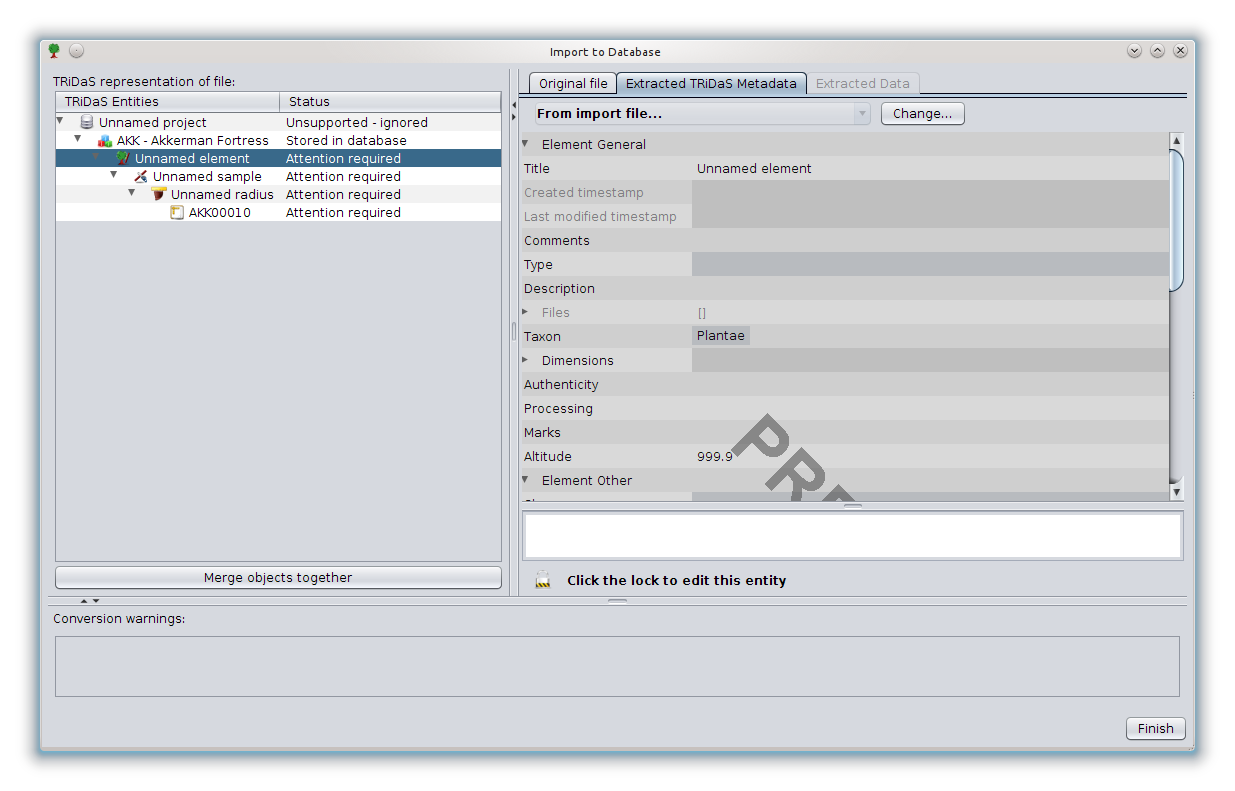
\includegraphics[width=0.95\textwidth]{Images/importdata1.png}
    \caption{Screenshot of the import dialog.  The screen is divided into three main sections.  The top left contains a TRiDaS representation of the data file that is being imported.  The top right panel contains the metadata gleaned from each of these TRiDaS entities.  At the bottom of the screen is a table containing any warnings associated with the conversion.  In this case there are no warnings. }
    \label{fig:import}
\end{figure}

Once you have picked the file you'd like to import, an import dialog screen similar to that shown in figure \ref{fig:import} is displayed. The dialog is divided into three main sections: TRiDaS hierarchy (top left); Data viewer (top right); and Warnings panel (bottom).   

The TRiDaS hierarchy panel contains a representation of the file being imported according to the TRiDaS data model.  This table also contains a status column to indicate whether input is required from the user.  The two main status options are `Stored in database'--to indicate that the entity is already stored in the Tellervo database--and `Attention required'--to indicate the entity needs to be cleaned up by the user.  

The data viewer panel on the top right of the dialog contains three tabs.  The first gives a standard text editor representation of the file being imported.  Note that when errors are detected in the file, Tellervo will highlight, where possible, the portion of the file that is causing the problem.  The second tab contains a metadata editor for the current TRiDaS entity.  The third tab contains a viewer for ring width values if the entity selected is a measurment series.

The warnings panel at the bottom of the screen contains a list of any warnings that have occurred during the conversion process.  There can be many issues when reading legacy data files, for instance some files do not contain information on the measurement units used.  In this case Tellervo will make an assumption and warn the user.  It is important to understand the assumptions and warnings provided by Tellervo in this panel otherwise erroneous (meta)data may be imported.

\subsection{Importing when entities are already in the database}
If you already have the object, element, sample and radius entities entered in your Tellervo database for the series you are trying to import the import process largely involves picking the relevant entities from the database.  

First of all, click the most senior entity in the TRiDaS hierarchy on the left which has the status `Attention required'.  The dialog will update and the limited metadata that Tellervo has been able to glean from the file will be shown on the right.  As we already have all the information we need about this entity stored in the database, we simply need to replace this `skinny' entity with the rich one we have in the database.  This is down by clicking the `Change' button in the metadata viewer on the right and then by choosing the correct entity from the pull down menu.  Click the choose button and the swap will be complete.  Notice now that in the TRiDaS hierarchy that the status for this entity is changed to `Stored in database'.  You can continue working down the hierarchy in a similar way.

\subsection{Importing when entities are not in the database}
If you are importing a file that contains entities that you \emph{don't} already have stored in your database, then you will need to clean them up and save them.   Select the most senior entity that needs to be imported in the TRiDaS hierarchy panel.  The metadata gleaned by Tellervo from the legacy file will be previewed in the metadata panel on the right.  Next, click the `lock' icon at the bottom of the metadata panel and the metadata will become editable.  You will then need to spend some time filling out and cleaning up the metadata for this entity.  

An important part of the import process is the standardization of the metadata.  Take for instance the example of the taxon.  Most legacy files have some method for indicating what species a file is about, but most do so by allowing the user to type in a free text field.  The TRiCYCLE libraries that Tellervo uses are able to read such fields but the red oak (\textit{Quercus rubra}) may be represented in many ways: oak, red oak, Oak, \textit{Quercus}, \textit{Quercus} sp., \textit{Quercus rubra}, QUER etc, not to mention the scientific synonyms for the species e.g. \textit{Quercus acerifolia}, \textit{Quercus ambigua}, \textit{Quercus angulizana} to name but a few.  Many users would know that these represent the same species, but if you were to query your database for Quercus rubra, you would miss records stored under the other names.  It is therefore essential to standardize them to a single dictionary of terms.  In the case of species names, Tellervo use the Catalogue of Life \citep{col}.  There are a number of similar enumerated metadata fields in Tellervo, each indicated by a pull down menu.  When importing, these fields will be populated with the non-normalized term read by Tellervo, but to successfully import the entity into the database, you will need to choose the corresponding `controlled vocabulary' term from the pull down menu.  

Once you have cleaned and normalized your metadata, you need to press the `Save changes' button to upload the entity into the database.  You will be provided with an error message if you have missed any mandatory fields, or if you have not normalized all the data to terms stored in the Tellervo dictionaries.  Once you have successfully saved the entity, the TRiDaS hierarchy on the left will be updated so the status reads `Stored in database'.  You will then need to work your way through the remaining entities to finish importing the file.

\subsection{Speeding up the process}
Manually choosing the relevant entry for each entity is quite a frustrating and time consuming task.  When importing a file containing multiple series, the task is compounded by the fact that Tellervo will often place the series into separate hierarchies.  Unfortunately, many legacy file formats do not contain enough information to enable Tellervo to determine whether they are from the same or different objects.  To be on the safe side, Tellervo therefore places them in separate `unknown' objects.  Rather that manually specifying the correct object repeatedly, you can use the `merge objects' button to do this for you.  You need then only pick the correct object from the database once.



\section{Exporting graphs}
\index{Export!Graphs}



\section{Exporting maps}
\index{Export!Maps}
\index{Mapping!Export|see{Export -- Maps}}


